\section{Forecasting}
\subsection{Business Series}
Adopting ARIMA$(1, 1, 2)(2, 1, 0)_4$ as the fitted model for the Business series, forecasts of the number of business trips for the next 8 quarters (2018 Q1 to 2019 Q4) are obtained using the $\texttt{predict}$ function.
\vspace{-0.4cm}
\begin{figure}[H]
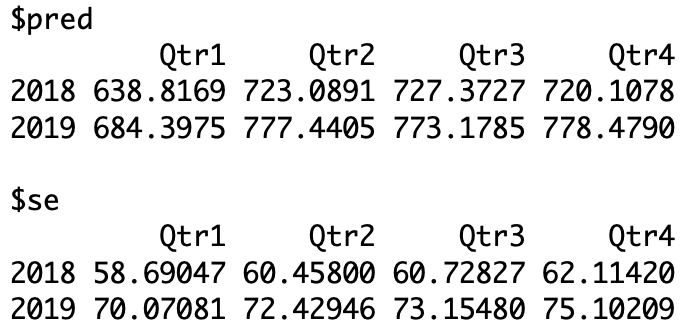
\includegraphics[width=0.4\linewidth]{fig/y1pred.png}
\end{figure}

\vspace{-0.4cm}
\begin{figure}[H]
    \centering
    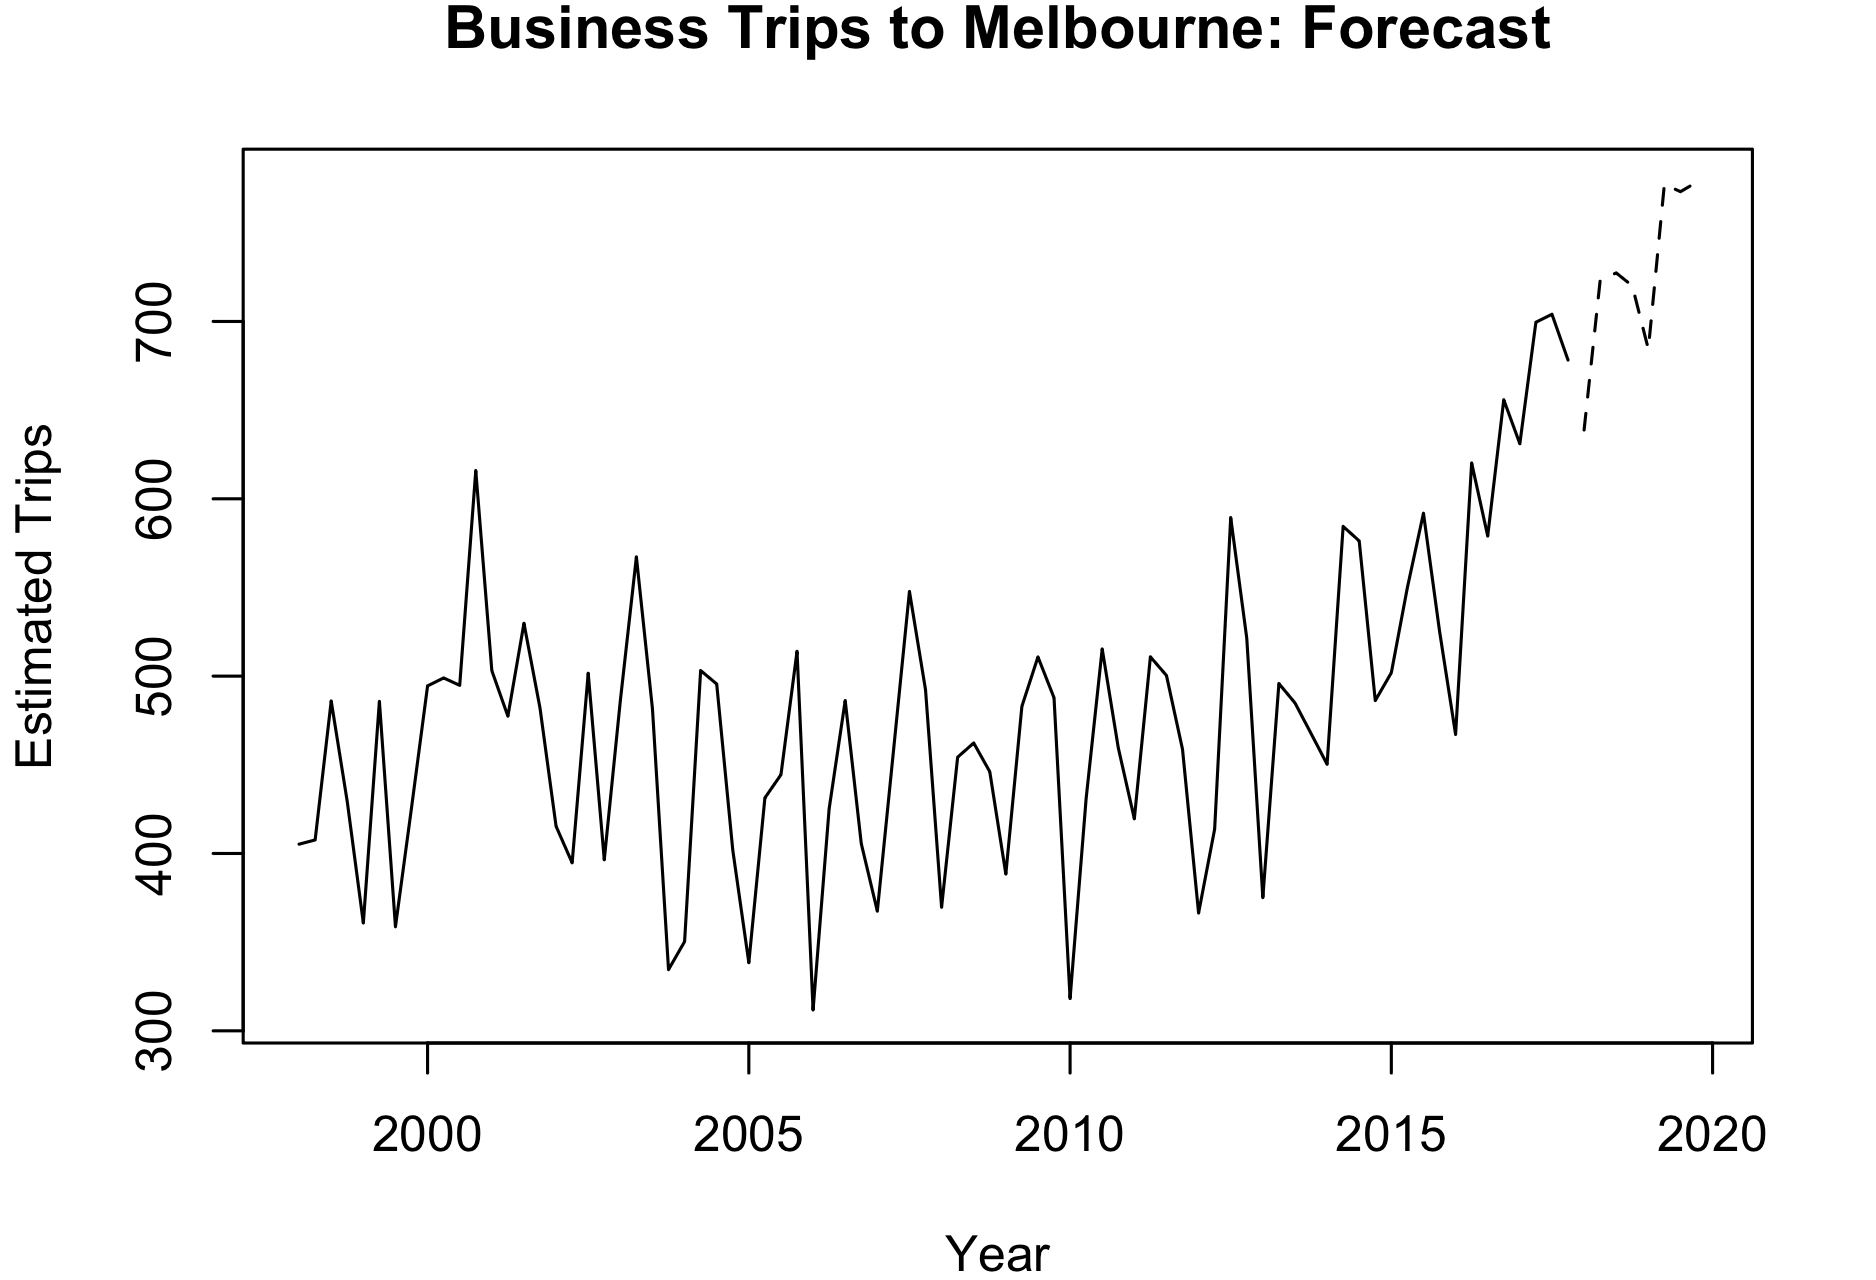
\includegraphics[width=0.65\linewidth]{fig/y1frc.png}
\end{figure}

\noindent The forecasts continue the upward trend and quarterly seasonal pattern established over the observation period, with trips lowest in Q1 of each forecast year and highest around Q2–Q3, consistent with the seasonal pattern identified previously.

\begin{table}[H]
\centering
\begin{tabular}{lccc}
\hline
Time & Forecast & Lower 95\% & Upper 95\% \\
\hline
2018 Q1 & 638.8 & 523.8 & 753.8 \\
2018 Q2 & 723.1 & 604.6 & 841.6 \\
2018 Q3 & 727.4 & 608.3 & 846.4 \\
2018 Q4 & 720.1 & 598.4 & 841.9 \\
2019 Q1 & 684.4 & 547.1 & 821.7 \\
2019 Q2 & 777.4 & 635.5 & 919.4 \\
2019 Q3 & 773.2 & 629.8 & 916.6 \\
2019 Q4 & 778.5 & 631.3 & 925.7 \\
\hline
\end{tabular}
\end{table}

\noindent The prediction intervals increased steadily, from approximately 230 trips at one-quarter ahead to about 294 trips at eight-quarters ahead, reflecting the greater uncertainty attached to forecasts made further into the future.

\noindent These forecasts assume that the trend and seasonal pattern observed up to 2017 Q4 continue unchanged. Any structural changes in the tourism market, such as shifts in business travel behaviour, may cause actual values to deviate from these forecasts.


\subsection{Holiday Series}

Adopting the fitted seasonal ARIMA model for the Holiday series, forecasts of the number of holiday trips for the next 8 quarters (2018 Q1 to 2019 Q4) are obtained using the $\texttt{predict}$ function.

\vspace{-0.4cm}
\begin{figure}[H]
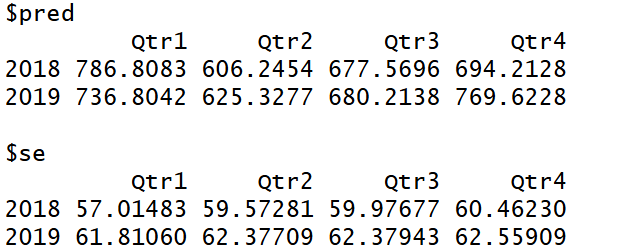
\includegraphics[width=0.4\linewidth]{fig/y2pred.png}
\end{figure}

\vspace{-0.4cm}
\begin{figure}[H]
    \centering
    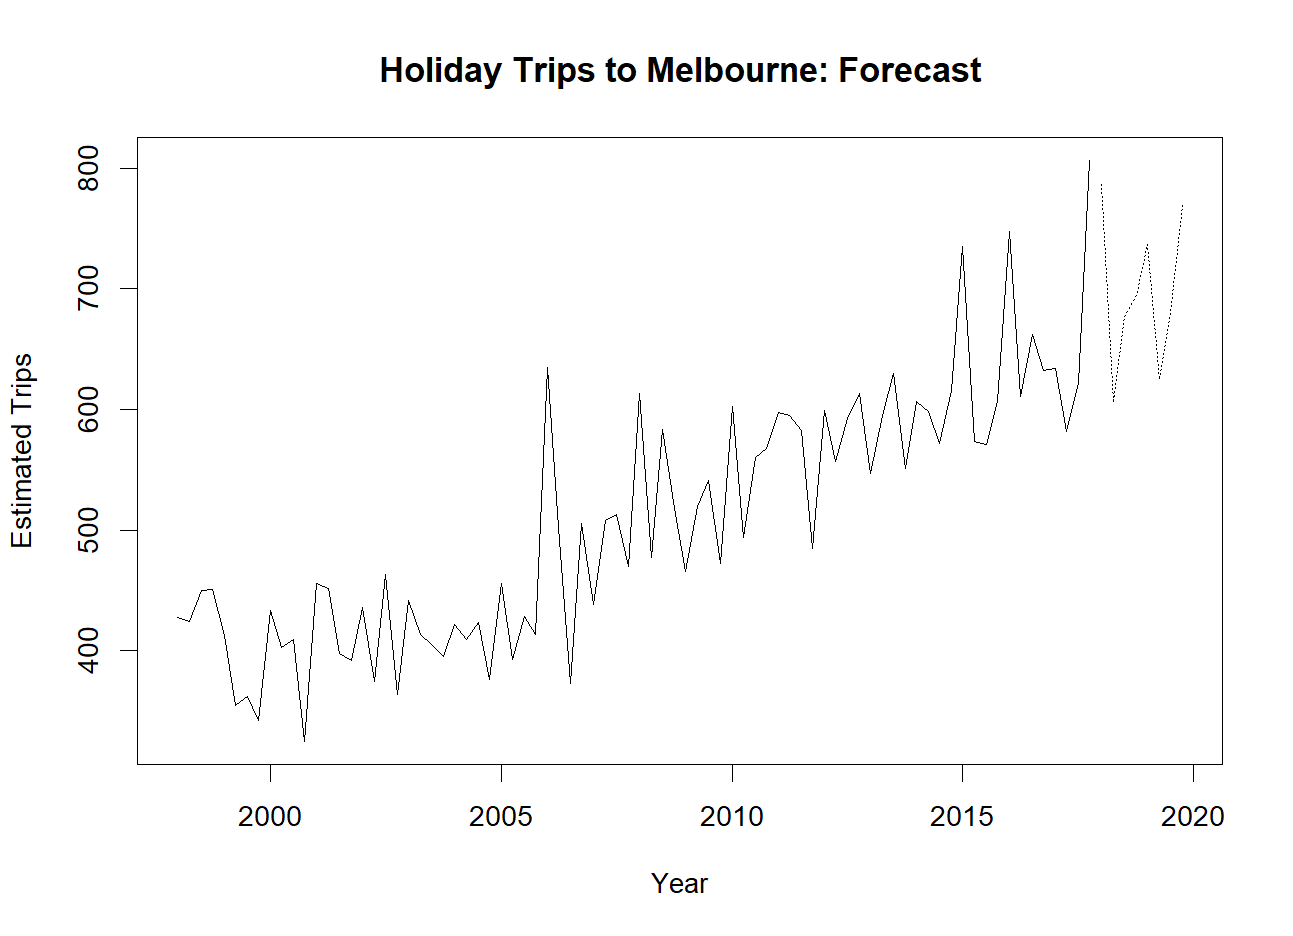
\includegraphics[width=0.7\linewidth]{fig/y2frc.png}
\end{figure}

\noindent The forecasts preserve the seasonal pattern observed in the Holiday series. The predicted values show a recurring quarterly pattern, with higher numbers of holiday trips occurring around Q1 and Q4, while relatively lower values are observed in Q2. This behaviour is consistent with the seasonal variation identified from the previous time series analysis.

\begin{table}[H]
\centering
\begin{tabular}{lccc}
\hline
Time & Forecast & Lower 95\% & Upper 95\% \\
\hline
2018 Q1 & 786.8 & 675.1 & 898.5 \\
2018 Q2 & 606.2 & 489.5 & 723.0 \\
2018 Q3 & 677.6 & 559.9 & 795.2 \\
2018 Q4 & 694.2 & 575.7 & 812.7 \\
2019 Q1 & 736.8 & 615.6 & 858.0 \\
2019 Q2 & 625.3 & 503.1 & 747.6 \\
2019 Q3 & 680.2 & 557.9 & 802.5 \\
2019 Q4 & 769.6 & 646.9 & 892.3 \\
\hline
\end{tabular}
\end{table}

\noindent The prediction intervals become wider as the forecast horizon increases. The interval width increases from approximately 223 trips for the first forecast quarter to around 245 trips for the final forecast quarter, indicating increasing uncertainty for forecasts further into the future.

\noindent These forecasts assume that the historical seasonal pattern of holiday travel continues unchanged. However, future holiday travel demand may be influenced by external factors such as economic conditions, tourism trends, and unexpected events, which may cause actual values to deviate from the forecasts.
